\documentclass{beamer}
\usetheme[white]{Wisconsin}
\usepackage{wrapfig}
\usepackage{longtable}
\usepackage{listings}
\usepackage{color}
\usepackage{graphicx}
%% Renumber appendix
\usepackage{appendixnumberbeamer}
%% The amssymb package provides various useful mathematical symbols
\usepackage{amssymb}
%% The amsthm package provides extended theorem environments
\usepackage{amsthm} \usepackage{amsmath}
\usepackage[mathcal]{euscript} \usepackage{color}
\usepackage{textcomp}
\usepackage{algorithm,algorithmic}
\usepackage[absolute,overlay]{textpos}
  \setlength{\TPHorizModule}{1mm}
  \setlength{\TPVertModule}{1mm}
\definecolor{listinggray}{gray}{0.9}
\definecolor{lbcolor}{rgb}{0.9,0.9,0.9}
\lstset{
  backgroundcolor=\color{lbcolor},
  tabsize=4,
  rulecolor=,
  language=c++,
  basicstyle=\scriptsize,
  upquote=true,
  aboveskip={1.5\baselineskip},
  columns=fixed,
  showstringspaces=false,
  extendedchars=true,
  breaklines=true,
  prebreak =
  \raisebox{0ex}[0ex][0ex]{\ensuremath{\hookleftarrow}},
  frame=single,
  showtabs=false,
  showspaces=false,
  showstringspaces=false,
  identifierstyle=\ttfamily,
  keywordstyle=\color[rgb]{0,0,1},
  commentstyle=\color[rgb]{0.133,0.545,0.133},
  stringstyle=\color[rgb]{0.627,0.126,0.941},
}
\AtBeginSection[]
{
  \begin{frame}<beamer>
    \frametitle{Outline}
    \tableofcontents[currentsection]
  \end{frame}
}

\newcommand{\backupbegin}{
   \newcounter{framenumberappendix}
   \setcounter{framenumberappendix}{\value{framenumber}}
}
\newcommand{\backupend}{
   \addtocounter{framenumberappendix}{-\value{framenumber}}
   \addtocounter{framenumber}{\value{framenumberappendix}} 
}

%% colors
\setbeamercolor{boxheadcolor}{fg=white,bg=UWRed}
\setbeamercolor{boxbodycolor}{fg=black,bg=white}

\setbeamerfont{block body}{size=\footnotesize}

%%---------------------------------------------------------------------------%%
\author{Alex P. Robinson
    \\ Engineering Physics Department
    \\ University of Wisconsin - Madison
    \\ Group Meeting
}

\date{\today}
\title{Overview and Testing of TPOR 1.0.0} 
\begin{document}
\maketitle
%%---------------------------------------------------------------------------%%
%% Overview
%%---------------------------------------------------------------------------%%
\begin{frame}{Outline}

  \tableofcontents

\end{frame}

%%---------------------------------------------------------------------------%%
\section{Optimization and the Greedy Heuristic}
%%---------------------------------------------------------------------------%%
\begin{frame}{The Optimization Problem}

  \begin{itemize}
    \item In computer science, optimization problems belong to a class of 
      problems known as NP-complete (Dasgupta, 2006).
      \medskip
    \item Typically, the only way to solve an NP-complete problem exactly is an
      exhaustive search (Dasgupta, 2006).
      \medskip
    \item Any method to reduce the search space based on some additional info 
      or experience is called a heuristic.
      \medskip
    \item Heuristics are not guaranteed to find an optimal solution but in
      some cases, the worst case ``distance'' from optimal is known 
      (Chvatal, 1979).
  \end{itemize}

\end{frame}

%%---------------------------------------------------------------------------%%
\begin{frame}{The Greedy Heuristic}

  \begin{itemize}
    \item The greedy heuristic is a well know heuristic in the computer 
      science community for solving a variety of optimization problems
      (Chvatal, 1979).
      \medskip
    \item It simply requires one to make the locally optimal choice, based on 
      some criterion, at each step of solution construction.
      \medskip
    \item All of the algorithms for interstitial prostate brachytherapy
      treatment planning optimization that will be discussed are greedy 
      heuristics.
      \medskip
    \item The decision criterion for each of these algorithms incorporates
      adjoint dose data related to the patient.
  \end{itemize}
  
\end{frame}

%%---------------------------------------------------------------------------%%
\section{Greedy Heuristics for Interstitial Prostate Brachytherapy}
%%---------------------------------------------------------------------------%%
\begin{frame}{The Basic Position Ranking Metric}
  
  \begin{itemize}
    \item The most basic quantity used for evaluating the desirability of a
      brachytherapy seed positions is the adjoint ratio.
      \medskip
    \item The adjoint ratio essentially indicates the amount of dose delivered 
      to healthy tissue relative to the amount of dose delivered to the target
      tissue (given weights of unity). 
      \medskip
    \item This quantity is static and can thus be considered a property of a
      potential seed position.
      \medskip
  \end{itemize}
  
  \begin{beamerboxesrounded}[upper=boxheadcolor,lower=boxbodycolor,shadow=true]{Adjoint Ratio}
    \begin{equation*}
      C_{i} = \frac{w_{ur}\phi_{ur,i}^{\dagger}+w_{re}\phi_{re,i}^{\dagger}+w_{ma}\phi_{ma,i}^{\dagger}}{w_{ta}\phi_{ta,i}^{\dagger}}
    \end{equation*}
  \end{beamerboxesrounded}
  
\end{frame}

%%---------------------------------------------------------------------------%%
\begin{frame}{Midplane Adjoint Flux Distributions for Tissue ROIs}

  \begin{textblock}{20}(2,10)
    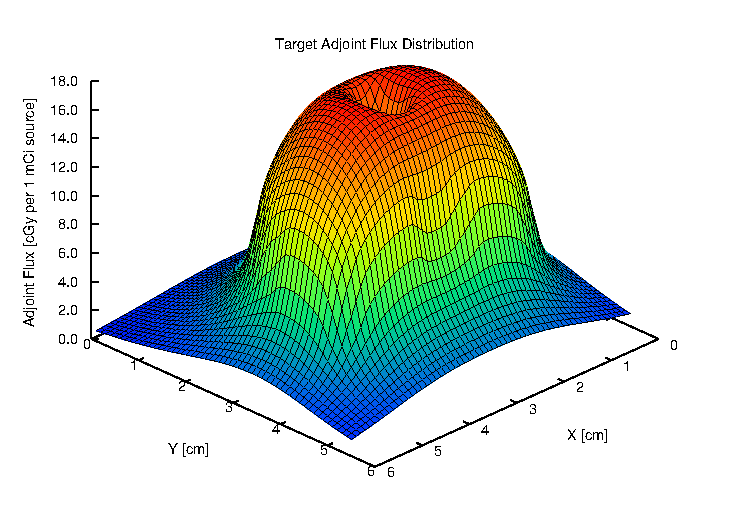
\includegraphics[width=2.5in]{figures/Target_adjoint_flux-midplane.pdf}
  \end{textblock}

  \begin{textblock}{20}(65,10)
    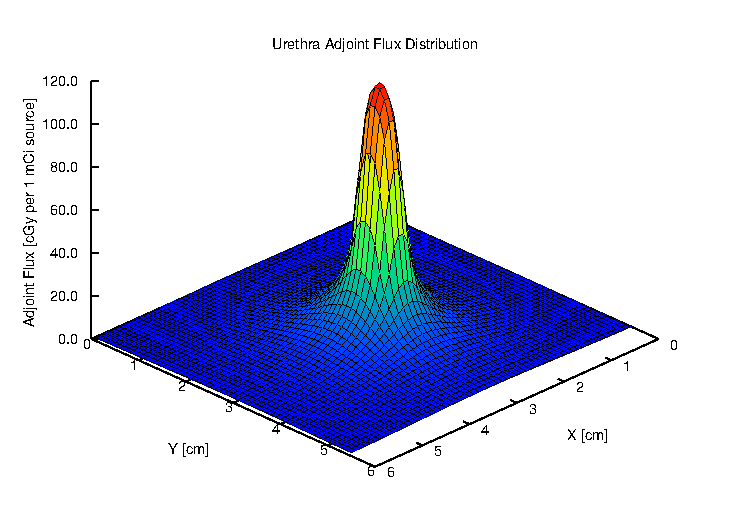
\includegraphics[width=2.5in]{figures/Urethra_adjoint_flux-midplane.pdf}
  \end{textblock}

  \begin{textblock}{20}(2,53)
    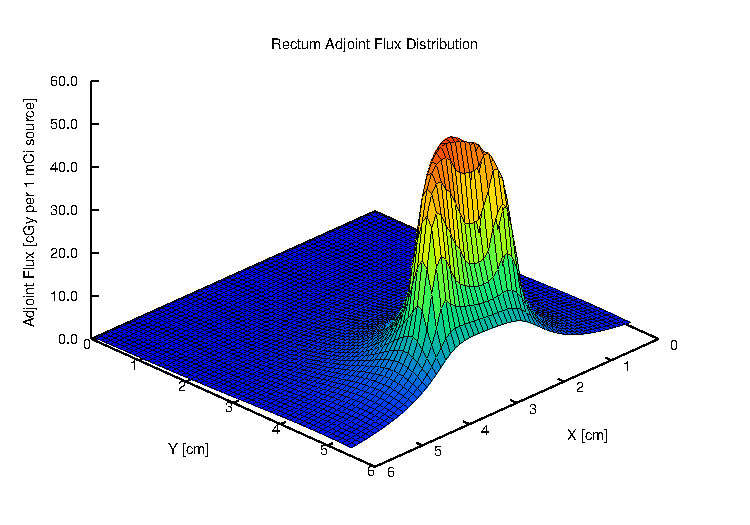
\includegraphics[width=2.5in]{figures/Rectum_adjoint_flux-midplane.pdf}
  \end{textblock}

  \begin{textblock}{20}(65,53)
    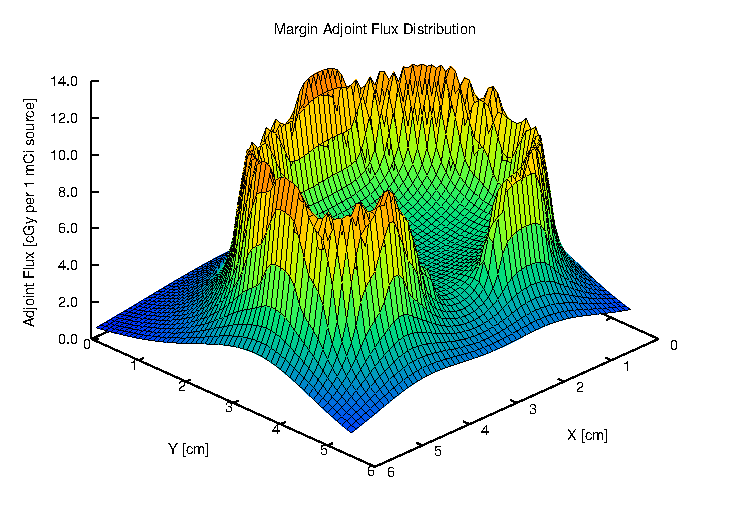
\includegraphics[width=2.5in]{figures/Margin_adjoint_flux-midplane.pdf}
  \end{textblock}

\end{frame}

%%---------------------------------------------------------------------------%%
\begin{frame}{Adjoint Ratios at Z= 1.25, 2.25, 3.25, 4.25 cm}

  \begin{textblock}{20}(2,10)
    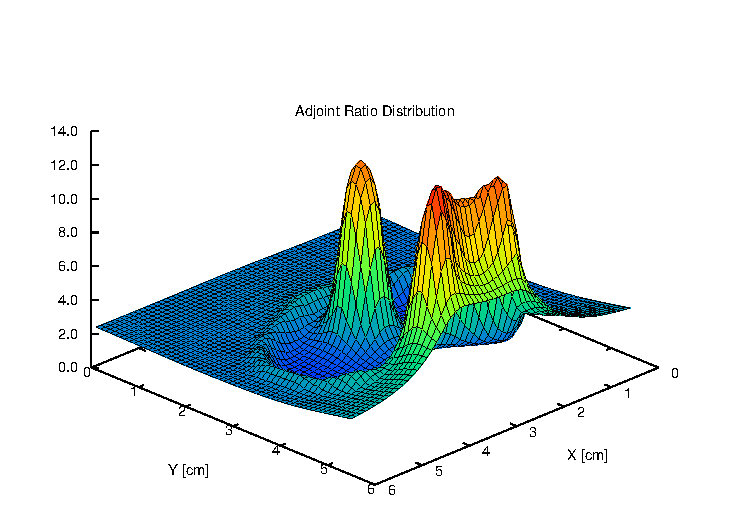
\includegraphics[width=2.5in]{figures/adjoint_ratio-slice3.pdf}
  \end{textblock}

  \begin{textblock}{20}(65,10)
    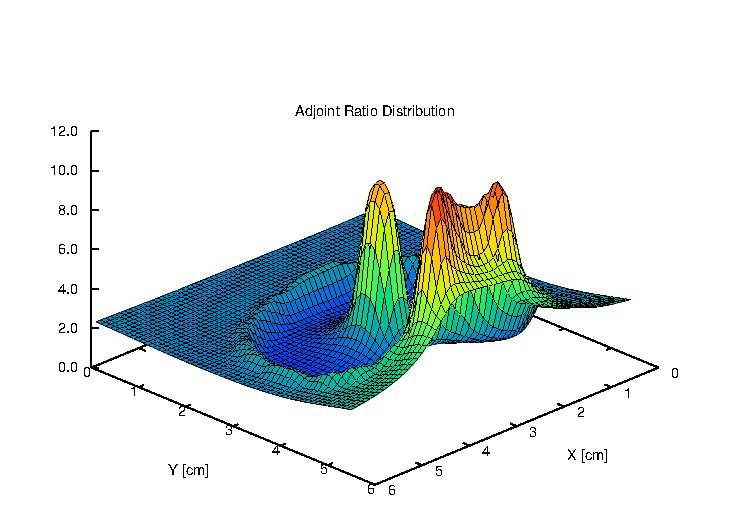
\includegraphics[width=2.5in]{figures/adjoint_ratio-slice5.pdf}
  \end{textblock}

  \begin{textblock}{20}(2,53)
    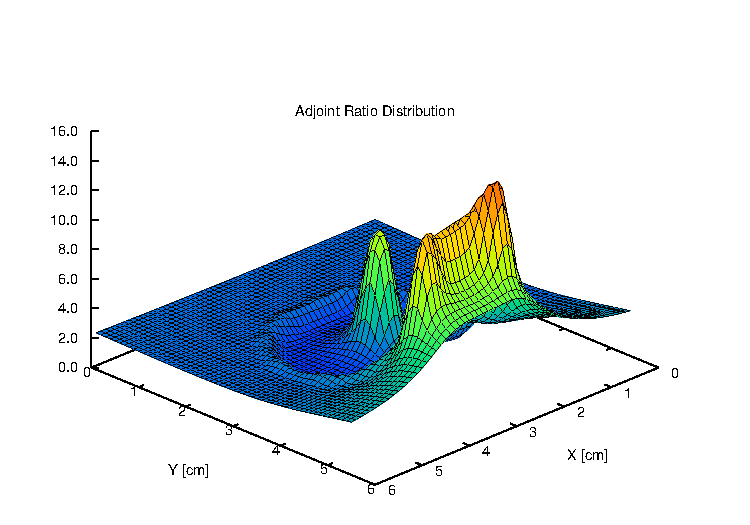
\includegraphics[width=2.5in]{figures/adjoint_ratio-slice7.pdf}
  \end{textblock}

  \begin{textblock}{20}(65,53)
    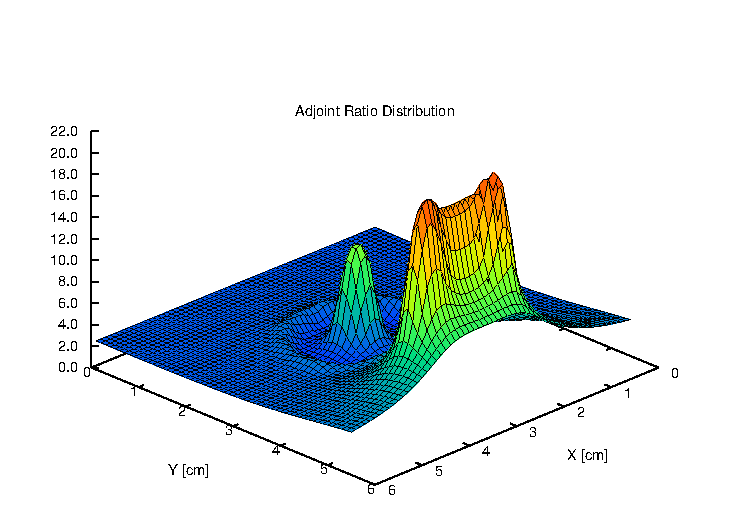
\includegraphics[width=2.5in]{figures/adjoint_ratio-slice9.pdf}
  \end{textblock}

\end{frame}

%%---------------------------------------------------------------------------%%
\begin{frame}{Adjoint Ratios on Needles at Z= 1.25, 2.25, 3.25, 4.25 cm}

  \begin{textblock}{20}(2,10)
    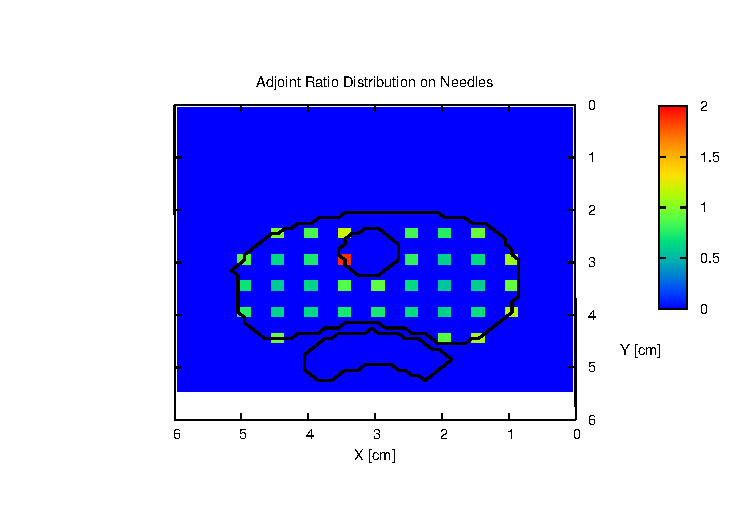
\includegraphics[width=2.5in]{figures/adjoint_ratio_needles-slice3.pdf}
  \end{textblock}

  \begin{textblock}{20}(65,10)
    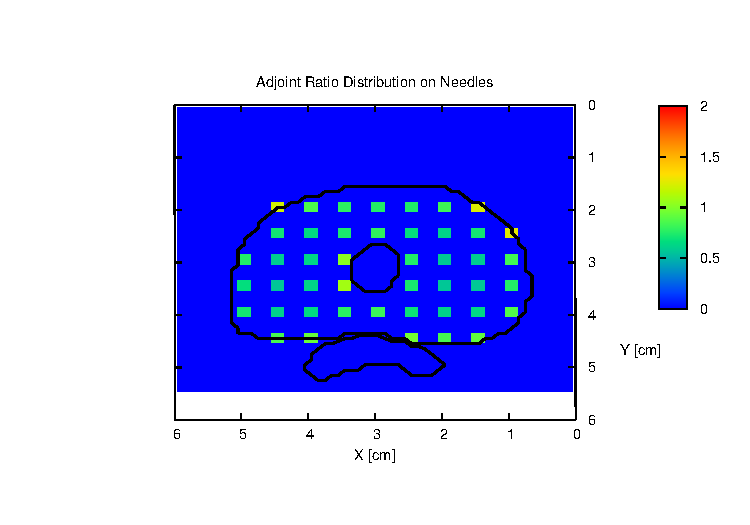
\includegraphics[width=2.5in]{figures/adjoint_ratio_needles-slice5.pdf}
  \end{textblock}

  \begin{textblock}{20}(2,53)
    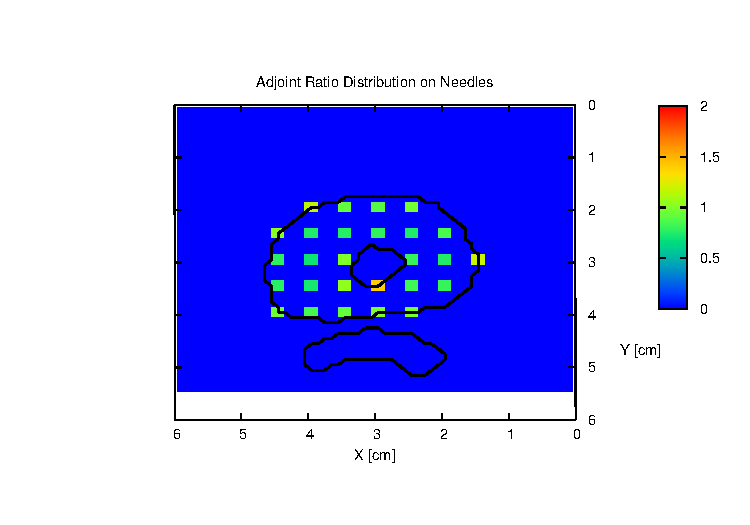
\includegraphics[width=2.5in]{figures/adjoint_ratio_needles-slice7.pdf}
  \end{textblock}

  \begin{textblock}{20}(65,53)
    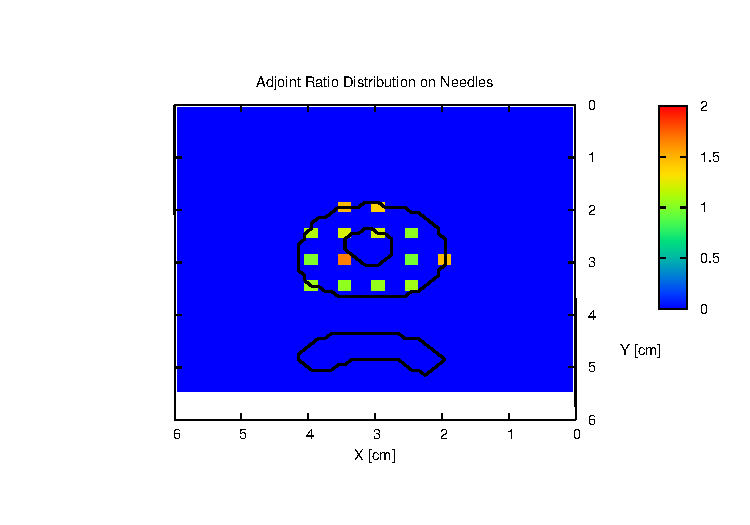
\includegraphics[width=2.5in]{figures/adjoint_ratio_needles-slice9.pdf}
  \end{textblock}
  
\end{frame}

%%---------------------------------------------------------------------------%%
\begin{frame}{Limitations of the Adjoint Ratio}

  \begin{textblock}{117}(4,15)
    \begin{itemize}
      \item Using the adjoint ratio as the sole criterion for choosing a seed
        position will result in seeds being clustered at low points along a 
        needle.
        \medskip
      \item A practical criterion needs to include additional information that
        prevents seeds from clustering.
    \end{itemize}
  \end{textblock}

  \begin{textblock}{20}(25,45)
    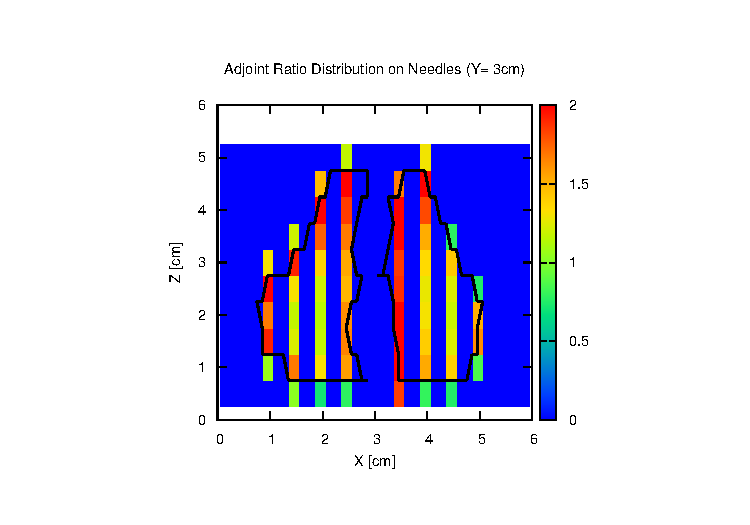
\includegraphics[width=3in]{figures/adjoint_ratio_needles-yslice.pdf}
  \end{textblock}

\end{frame}

%%---------------------------------------------------------------------------%%
\subsection{The Iterative Isodose Exclusion Method}
%%---------------------------------------------------------------------------%%
\begin{frame}{The Iterative Isodose Exclusion Method\footnote{This method was developed by Sua Yoo(Yoo et al, 2003).} (IIEM)}
  
  \begin{textblock}{117}(4,15)
    \begin{itemize}
      \item This method prevents seeds from clustering by imposing an isodose
        constraint on the seed selection process.
        \medskip
      \item Even if a seed position has the lowest adjoint ratio, it will not
        be selected if the dose at that seed position from other selected seeds
        is greater than the constraint value\footnote{Figure courtesy of 
          (Yoo et al., 2003)}.
    \end{itemize}
  \end{textblock}

  \begin{textblock}{40}(30,45)
    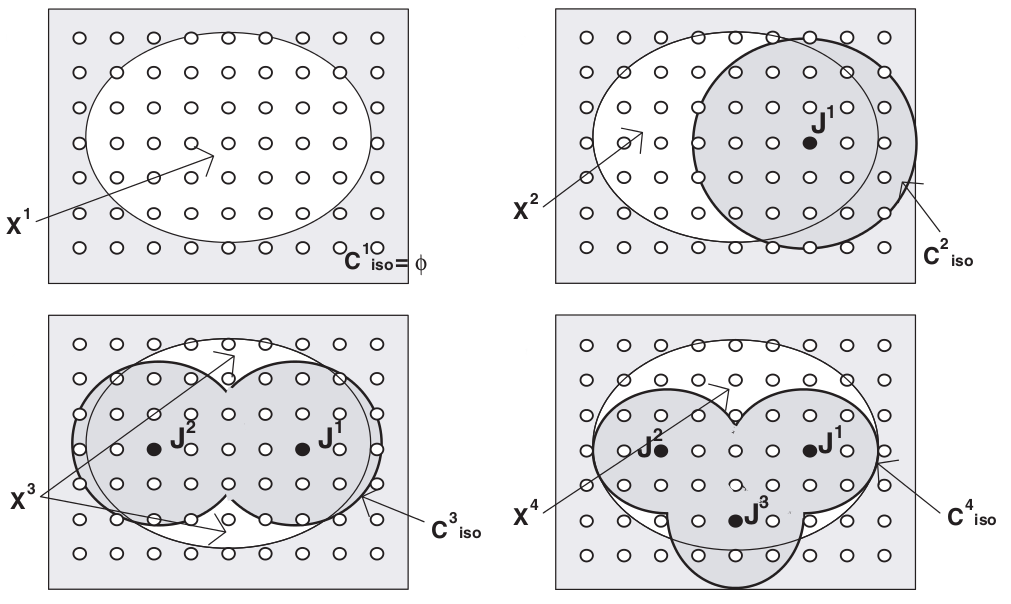
\includegraphics[width=2.5in]{figures/IIEM.png}
    
  \end{textblock}
  
\end{frame}

%%---------------------------------------------------------------------------%%
\begin{frame}{IIEM Pseudocode}
  
  \begin{itemize}
    \item \textit{Outer Iteration:} Select a needle goal
      \begin{itemize}
        \item \textbf{Inner Iteration A:} Select $\alpha$ for $C_{iso}^m$
          \begin{enumerate}
            \item Calculate $C_{iso}^m = \alpha *D_p*(m-1)$ for this step 
              (starting at m=1)\footnote{$D_p$ is the prescribed dose}
            \item Selected a seed by finding position with smallest 
              adjoint ratio and current dose less than $C_{iso}^m$
            \item If needle goal reached, continue to 
              \textbf{Inner Iteration B}, else select new $\alpha$
            \item If maximum $\alpha$ value reached, select new needle 
                  goal
          \end{enumerate}
          \medskip
        \item \textbf{Inner Iteration B:} Select $\beta$ for $C_{iso}^m$
          \begin{enumerate}
            \item Calculate $C_{iso}^m = \beta*D_p$ for this step
            \item Select a seed by finding position with smallest adjoint
              ratio and current dose less than $C_{iso}^m$
            \item If acceptable treatment plan achieved, end, else select a
              new $\beta$ value
            \item If maximum $\beta$ value reached, return to 
              \textbf{Inner Iteration A} and select new $\alpha$
          \end{enumerate}
      \end{itemize}
  \end{itemize}

\end{frame}

%%---------------------------------------------------------------------------%%
\subsection{The Dynamic-Weight Dose Multiplication Method}
%%---------------------------------------------------------------------------%%
\begin{frame}{The Dynamic-Weight Dose Mult. Method (DWDMM)\footnote{This method was developed by Vibha Chaswal (Chaswal et al., 2012)}}

  \begin{itemize}
      \item This method prevents seeds from clustering by utilizing a dynamic
        position value (weight). 
        \medskip
      \item After a seed has been selected, the adjoint ratio of all other
        seed positions is multiplied by the dose at its respective position. 
        \medskip
      \item The closer a seed position is to previously selected seeds, the
        larger its dynamic weight and the less likely it is to be picked.
    \end{itemize}

\end{frame}

%%---------------------------------------------------------------------------%%
\subsection{The Set Cover Method}
%%---------------------------------------------------------------------------%%
\begin{frame}{The Weighted Set Cover Problem}

  \begin{itemize}
    \item The set cover method for brachytherapy treatment planning is
      motivated by the greedy heuristic used to solve (approximately) the 
      weighted set cover problem
  \end{itemize}
  
  \medskip

  \begin{beamerboxesrounded}[upper=boxheadcolor,lower=boxbodycolor,shadow=true]
    {Problem Def. (Chvatal, 1979)}
    There are N sets and M elements. Each set $S_i$ has an associated cost 
    $c_i$. $I = \cup\left(S_j : 1 \leq j \leq N \right)$ contains all M 
    elements, while $J = \{S_1,S_2,...,S_N\}$ contains all sets. A subset $J^*$
    of $J$ is called a cover if $\cup\left(S_j : j \in J^* \right) = I$ with 
    corresponding cost $\sum\left(c_j : j \in J^*\right)$. 
    \textbf{Find a cover of minimum cost.}
  \end{beamerboxesrounded}
  
  \medskip

  \begin{beamerboxesrounded}[upper=boxheadcolor,lower=boxbodycolor,shadow=true]
    {Standard Greedy Heuristic (Chvatal, 1979)}
    \begin{enumerate}
      \item Set $J^* = \varnothing$
      \item If $S_j = \varnothing \ \forall j$ then stop: $J^*$ is a cover. 
        Otherwise find a subscript k minimizing the ratio 
        $\frac{c_j}{\mid S_j \mid}$.
      \item Add $S_k$ to $J^*$, replace each $S_j$ by $S_j - S_k$, return to step 
        2.
    \end{enumerate}
  \end{beamerboxesrounded}

\end{frame}

%%---------------------------------------------------------------------------%%
\begin{frame}{Properties of the Set Cover Greedy Heuristic}

  \begin{itemize}
    \item The greedy heuristic is a polynomial time algorithm
      \medskip
    \item The cost of the set cover found with this heuristic is guaranteed to
      be within $O(log(n))*C_{opt}$, where n is the number of elements and
      $C_{opt}$ is the cost of the optimal set cover (Chvatal, 1979).
      \medskip
    \item No polynomial time algorithm can get you a better approximation
      (Lund and Yankis, 1994).
  \end{itemize}

\end{frame}

%%---------------------------------------------------------------------------%%
\begin{frame}{Treatment Planning as a Set Covering}

  \begin{itemize}
    \item Treatment planning can be recast as a set covering problem:
      \medskip
      \begin{itemize}
        \item \textbf{$I$:} prostate mesh elements
        \item \textbf{${S_j}$:} seed position j, \textit{all} prostate mesh
          elements
        \item \textbf{$c_j$:} the adjoint ratio at the seed position.
        \item \textbf{$|S_j|$:} a new function is needed to evaluate the size 
          of set since all sets contain the same elements (departure from the 
          standard problem).
      \end{itemize}
  \end{itemize}

  \medskip

  \begin{beamerboxesrounded}[upper=boxheadcolor,lower=boxbodycolor,shadow=true]
    {Set Size Function}
    \begin{align}
      \mid S_j \mid & = \sum_{i}D_{new,i} \nonumber \\
      D_{new,i} & = 
      \begin{cases}
        (D_{future,i}-D_{current,i}) & \text{if } D_{future,i} < D_p \\
        (D_p - D_{current,i}) & \text{if } D_{future,i} > D_p \text{ and }
        D_{current,i} < D_p \\
        0 & \text{otherwise}
      \end{cases} \nonumber
    \end{align}
    $D_{current,i}$ is the dose at voxel $i$ from all previously placed seeds. 
    $D_{future,i}$ is the dose that will be at voxel $i$ if this seed is placed.
  \end{beamerboxesrounded}
  
\end{frame}

%%---------------------------------------------------------------------------%%
\begin{frame}{The Set Cover Method (SCM) Pseudocode}

  \begin{enumerate}
    \item Set $J^{*} = \varnothing$
      \medskip
    \item If an acceptable treatment plan has been achieved, end. Otherwise
      find a subscript k minimizing the ratio $\frac{c_j}{|S_j|}$.
      \medskip
    \item Add $S_k$ to $J^{*}$, return to step 2.
  \end{enumerate}

\end{frame}

%%---------------------------------------------------------------------------%%
\section{TPOR Library Overview}
%%---------------------------------------------------------------------------%%
\subsection{Code Flow}
%%---------------------------------------------------------------------------%%
\begin{frame}{TPOR Code Flow}

  \begin{figure}[h!]
    \begin{center}
      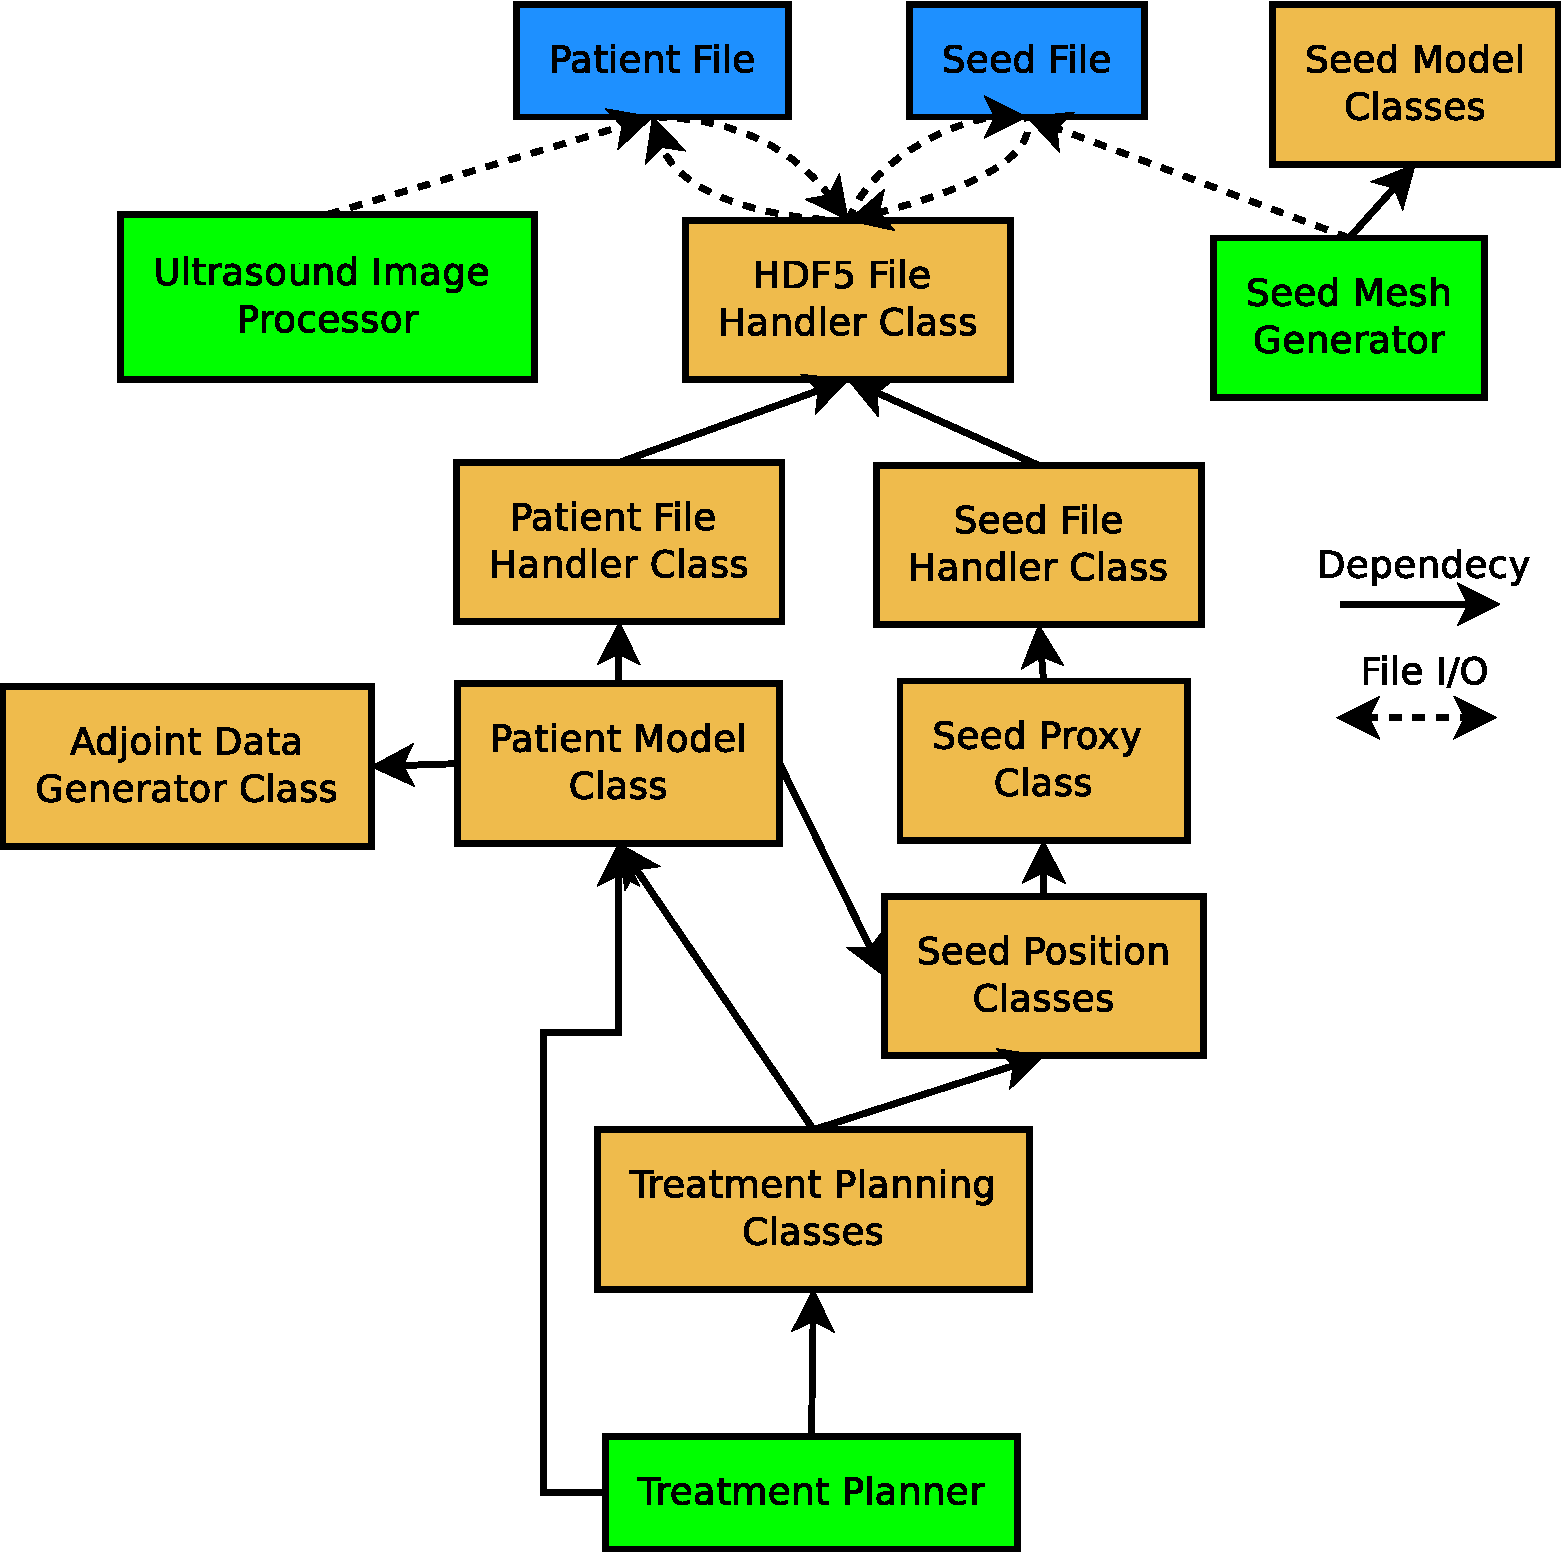
\includegraphics[width=3in,height=3in]{figures/TPOR_code_flow.pdf}
    \end{center}
  \end{figure}

\end{frame}

%%---------------------------------------------------------------------------%%
\subsection{Interface Files}
%%---------------------------------------------------------------------------%%
\begin{frame}{The Patient Interface File}
  
  \begin{itemize}
    \item All patient data is stored in a binary (HDF5) file.
      \medskip
    \item The patient data that can be found in this file are the patient organ
      masks, the organ volumes (approximate), the needle template, and the
      adjoint data associated with each seed and each organ.
      \medskip
    \item One should never interact or manipulate this file directly.
      \medskip
    \item Only use the \textit{Patient File Handler Class} to access data
      stored in this file.
      \medskip
    \item A python script has been written that allows one to create this file
      for a patient given an ultrasound image file.
  \end{itemize}

\end{frame}

%%---------------------------------------------------------------------------%%
\begin{frame}{The Seed Interface File}

  \begin{itemize}
    \item The dose distribution for a seed must be known in order to conduct
      a treatment planning optimization.
      \medskip
    \item The seed interface file (usually called 
      \textit{BrachytherapySeeds.h5}) stores the dose distribution of every
      low dose-rate (LDR) seed currently in production on a predefined mesh.
      \medskip
    \item One should never interact or manipulate this file directly.
      \medskip
    \item Only use the \textit{Seed File Handler Class} to access data stored
      in this file.
      \medskip
    \item A C++ program has be written that generates this file.
  \end{itemize}
  
\end{frame}

%%---------------------------------------------------------------------------%%
\subsection{Brachytherapy Seed Models}
%%---------------------------------------------------------------------------%%
\begin{frame}{The Brachytherapy Seed Models}

  \begin{itemize}
    \item All brachytherapy seeds are modeled using the recommendations from
      the TG-43 update for a line source approximation.
      \medskip
    \item The following brachytherapy seeds can be modeled by the TPOR library:
      \begin{itemize}
        \item Amersham 6711 ($I^{125}$)
        \item Amersham 9011 ($I^{125}$)
        \item Best 2301 ($I^{125}$)
        \item Best 2335 ($Pd^{103}$)
        \item Bebig I25.S06 ($I^{125}$)
        \item Theragenics 200 ($Pd^{103}$)
        \item Theragenics AgX100 ($I^{125}$)
        \item IsoAid IAI-125A ($I^{125}$)
        \item IsoAid IAPd-103A ($Pd^{103}$)
        \item SourceTech STM1251 ($I^{125}$)
        \item Nucletron 130.002 ($I^{125}$)
      \end{itemize}
  \end{itemize}
  
\end{frame}

%%---------------------------------------------------------------------------%%
\begin{frame}{The Seed Proxy Class}

  \begin{itemize}
    \item The class was created after profiling the TPOR library. 
      \medskip
    \item One of the original bottlenecks was the seed model class, which
      has to do many table look-ups and interpolations to get the dose at a 
      point.
      \medskip
    \item The seed proxy class simply stores the seed dose distribution mesh
      for a seed and looks up the value at a requested position. 
      \medskip
    \item Its class interface is nearly identical to the seed model class
      interface.
  \end{itemize}

\end{frame}

%%---------------------------------------------------------------------------%%
\subsection{Brachytherapy Seed Positions}
%%---------------------------------------------------------------------------%%
\begin{frame}{The Brachytherapy Seed Position Class}

  \begin{itemize}
    \item The brachytherapy seed position class only stores the most basic
      info needed by a treatment planning algorithm, i.e. the adjoint ratio
      (or weight) of a seed position. 
      \medskip
    \item The class also stores the seed type that would be placed at the 
      position, which facilities multispecies treatment planning.
      \medskip
    \item When a seed position is chosen, a member function must be called that
      maps the dose from the seed type to the patient organs.
      \medskip
    \item Only the IIEM treatment planning class uses this seed position class.
      \medskip
    \item Several more advanced seed position classes have also been written
      to provide the information needed by The DWDMM and SCM treatment planning
      classes.
  \end{itemize}
  
\end{frame}

%%---------------------------------------------------------------------------%%
\subsection{Patient Modeling}
%%---------------------------------------------------------------------------%%
\begin{frame}{The Patient Model}
  
  \begin{itemize}
    \item The patient model class stores the patient organ masks,
      needle template, prescribed dose, dose distribution and treatment plan.
      \medskip
    \item The class interface allows the treatment planning algorithms to 
      insert seeds into the patient model, determine properties of the 
      patient, and determine properties of the treatment plan.
      \medskip
    \item Upon completion of the treatment plan, the class can also print
      the treatment plan and other details that can be used to evaluate the
      quality of the plan.
  \end{itemize}
  
\end{frame}

%%---------------------------------------------------------------------------%%
\subsection{Treatment Planning Optimization}
%%---------------------------------------------------------------------------%%
\begin{frame}{The Treatment Planning Optimization Classes}

  \begin{itemize}
    \item All classes simply rely on the patient model class and one of the
      seed position classes.
      \medskip
    \item As seed positions are selected they are inserted into the patient
      model.
      \medskip
    \item Once the patient model indicates that an acceptable treatment plan
      has been achieved, the class releases the patient model for post 
      processing.
  \end{itemize}
  
\end{frame}

%%---------------------------------------------------------------------------%%
\section{Comparison Study}
%%---------------------------------------------------------------------------%%
\begin{frame}{A TPOR Comparison Study}
  
  \begin{itemize}
    \item Treatment plans for 16 patients were calculated using the three
      treatment planning algorithms currently in TPOR.
      \medskip
    \item All organ weights were set to one when calculating adjoint ratios.
      \medskip
    \item The quality of the plans as well as the optimization times were
      compared to draw conclusions about each of the algorithms.
      \medskip
    \item Much of the data is still being processed but DVH curves have been
      created.
  \end{itemize}

\end{frame}

%%---------------------------------------------------------------------------%%
\begin{frame}{Patient A DVH Curves}

  \begin{figure}[h!]
    \begin{center}
      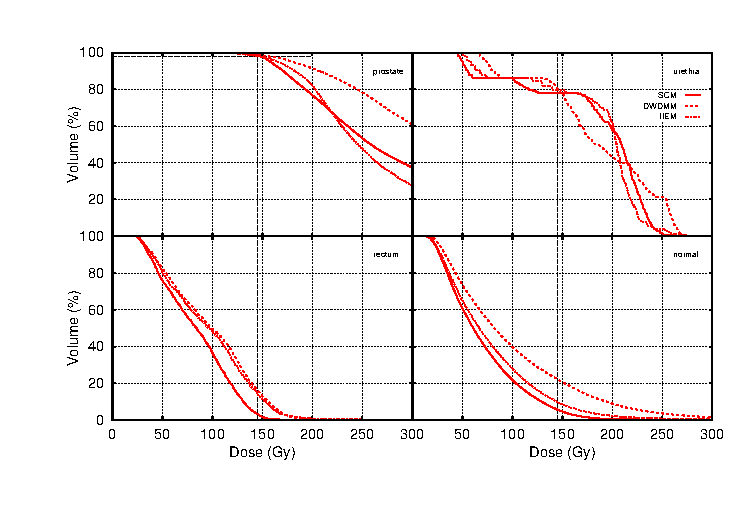
\includegraphics[width=4.3in]{figures/baron-all4x4.pdf}
    \end{center}
  \end{figure}

\end{frame}

%%---------------------------------------------------------------------------%%
\begin{frame}{Patient B DVH Curves}
  
  \begin{figure}[h!]
    \begin{center}
      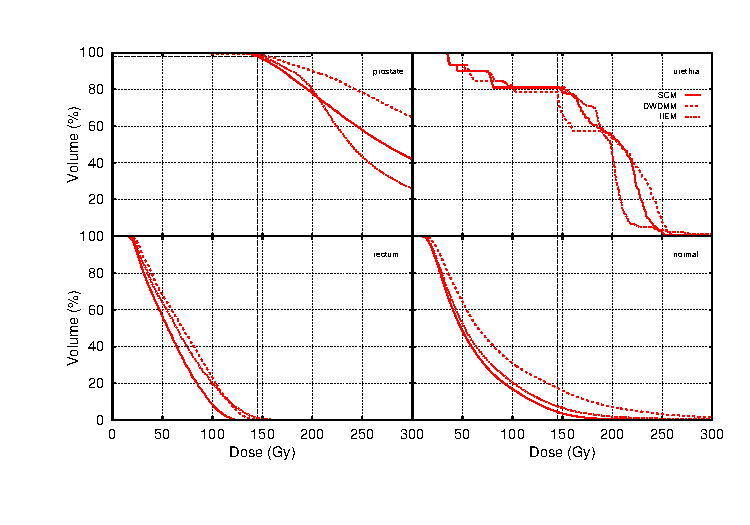
\includegraphics[width=4.3in]{figures/carlson-all4x4.pdf}
    \end{center}
  \end{figure}

\end{frame}

%%---------------------------------------------------------------------------%%
\begin{frame}{Patient C DVH Curves}
  
  \begin{figure}[h!]
    \begin{center}
      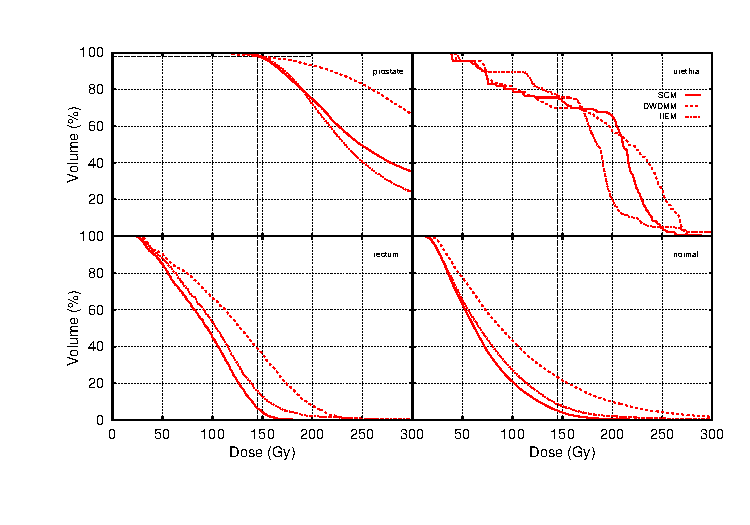
\includegraphics[width=4.3in]{figures/dittmar-all4x4.pdf}
    \end{center}
  \end{figure}

\end{frame}

%%---------------------------------------------------------------------------%%
\begin{frame}{Patient D DVH Curves}
  
  \begin{figure}[h!]
    \begin{center}
      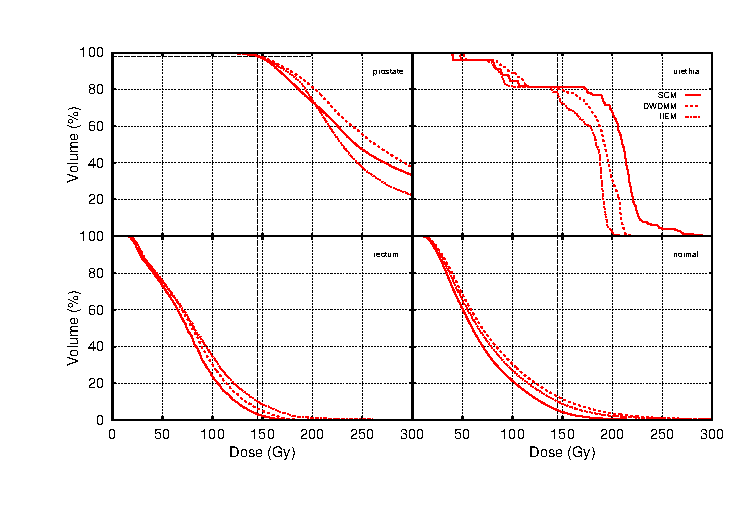
\includegraphics[width=4.3in]{figures/duckart-all4x4.pdf}
    \end{center}
  \end{figure}

\end{frame}

%%---------------------------------------------------------------------------%%
\begin{frame}{Patient E DVH Curves}
  
  \begin{figure}[h!]
    \begin{center}
      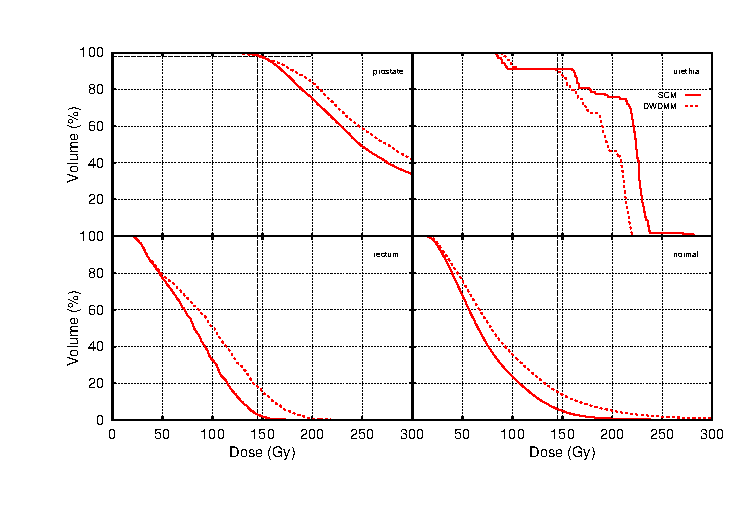
\includegraphics[width=4.3in]{figures/duffrin_tmp-all4x4.pdf}
    \end{center}
  \end{figure}

\end{frame}

%%---------------------------------------------------------------------------%%
\begin{frame}{Patient F DVH Curves}
  
  \begin{figure}[h!]
    \begin{center}
      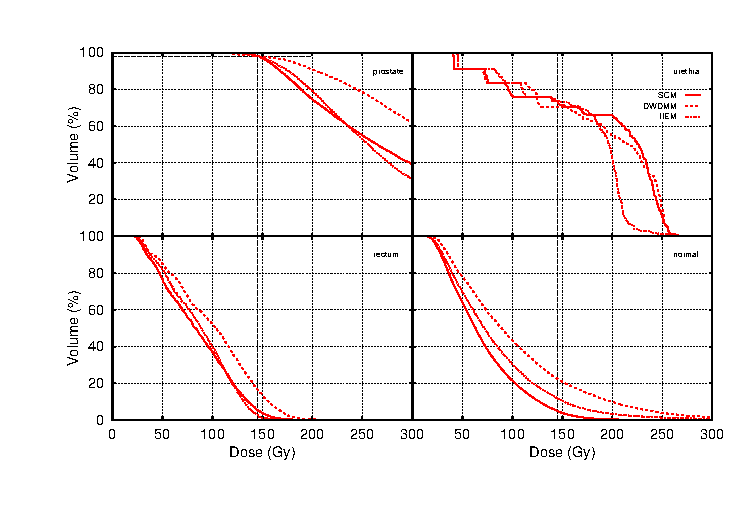
\includegraphics[width=4.3in]{figures/faber_9_11_98-all4x4.pdf}
    \end{center}
  \end{figure}

\end{frame}

%%---------------------------------------------------------------------------%%
\begin{frame}{Patient G DVH Curves}
  
  \begin{figure}[h!]
    \begin{center}
      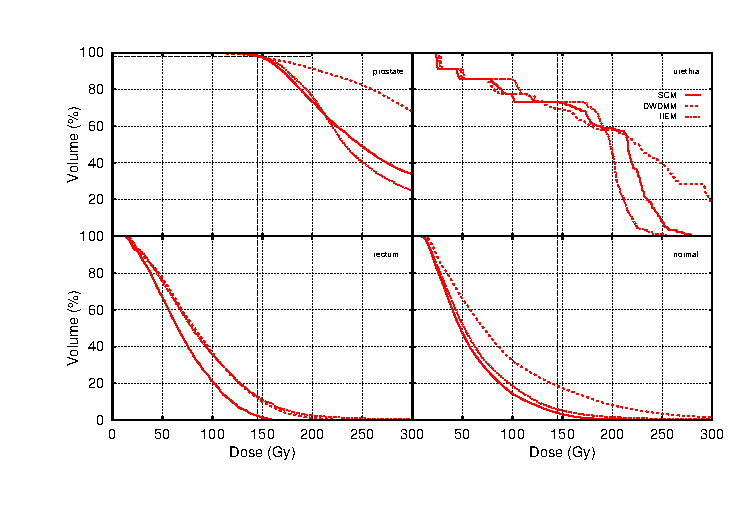
\includegraphics[width=4.3in]{figures/jkahle-all4x4.pdf}
    \end{center}
  \end{figure}

\end{frame}

%%---------------------------------------------------------------------------%%
\begin{frame}{Patient H DVH Curves}
  
  \begin{figure}[h!]
    \begin{center}
      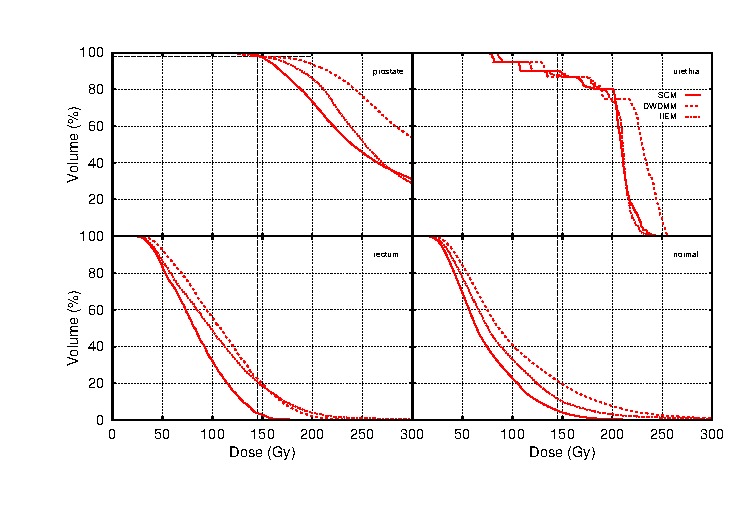
\includegraphics[width=4.3in]{figures/kahle-all4x4.pdf}
    \end{center}
  \end{figure}

\end{frame}

%%---------------------------------------------------------------------------%%
\begin{frame}{Patient I DVH Curves}
  
  \begin{figure}[h!]
    \begin{center}
      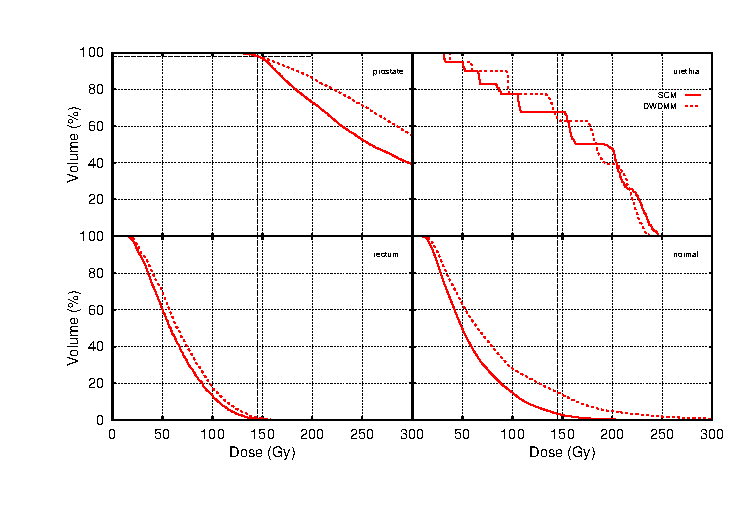
\includegraphics[width=4.3in]{figures/oestreicher-all4x4.pdf}
    \end{center}
  \end{figure}

\end{frame}

%%---------------------------------------------------------------------------%%
\begin{frame}{Patient J DVH Curves}
  
  \begin{figure}[h!]
    \begin{center}
      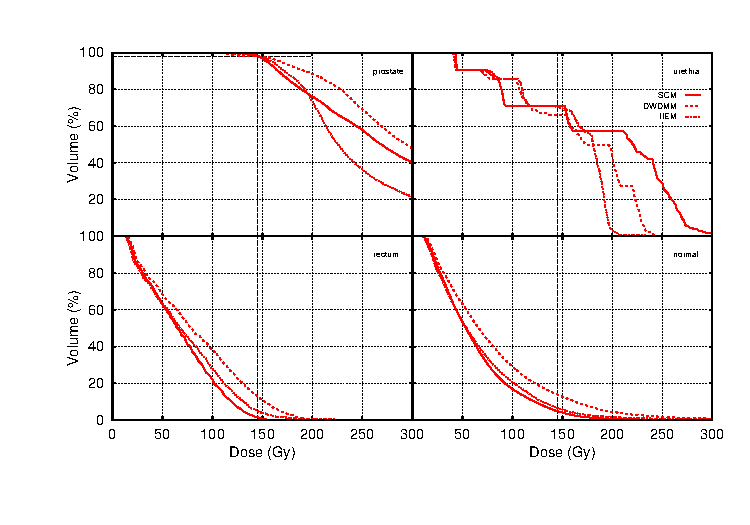
\includegraphics[width=4.3in]{figures/olson_us-all4x4.pdf}
    \end{center}
  \end{figure}

\end{frame}

%%---------------------------------------------------------------------------%%
\begin{frame}{Patient K DVH Curves}
  
  \begin{figure}[h!]
    \begin{center}
      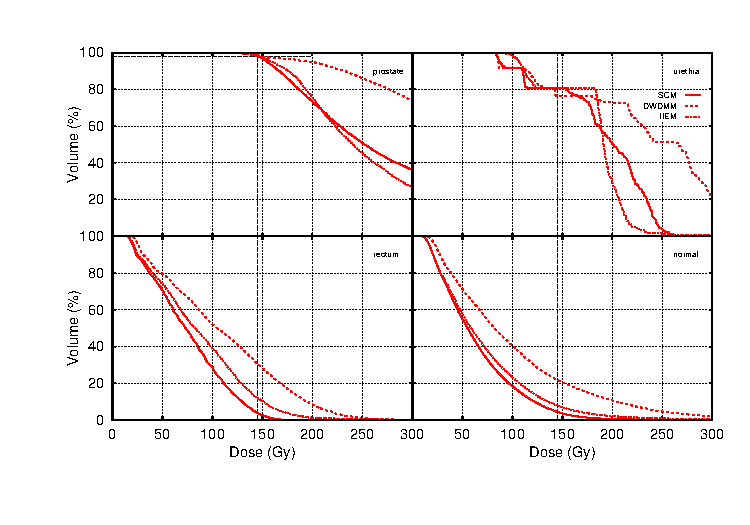
\includegraphics[width=4.3in]{figures/saupe_us-all4x4.pdf}
    \end{center}
  \end{figure}

\end{frame}

%%---------------------------------------------------------------------------%%
\begin{frame}{Patient L DVH Curves}
  
  \begin{figure}[h!]
    \begin{center}
      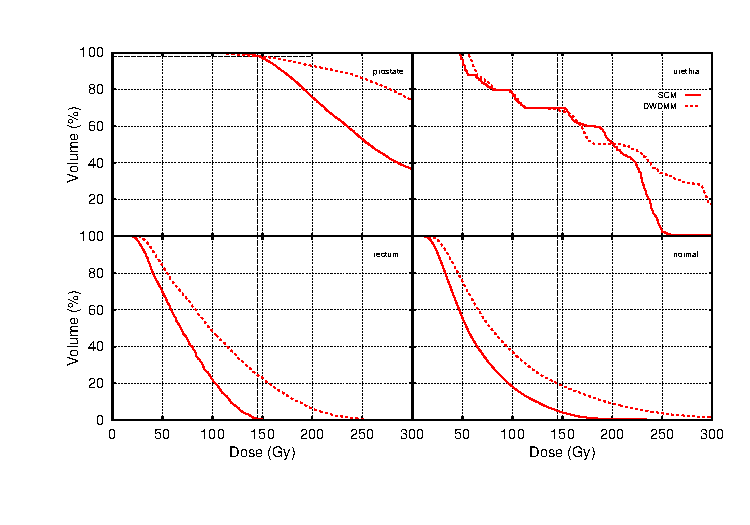
\includegraphics[width=4.3in]{figures/smieja-all4x4.pdf}
    \end{center}
  \end{figure}

\end{frame}

%%---------------------------------------------------------------------------%%
\begin{frame}{Patient M DVH Curves}
  
  \begin{figure}[h!]
    \begin{center}
      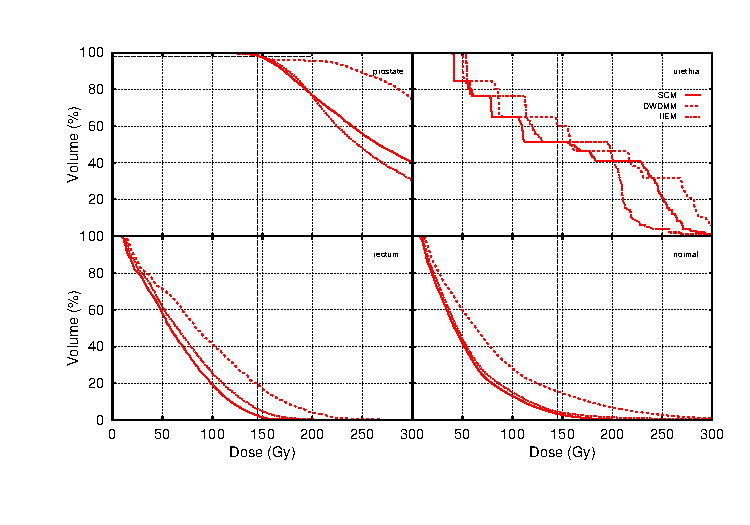
\includegraphics[width=4.3in]{figures/smith-all4x4.pdf}
    \end{center}
  \end{figure}

\end{frame}

%%---------------------------------------------------------------------------%%
\begin{frame}{Patient N DVH Curves}
  
  \begin{figure}[h!]
    \begin{center}
      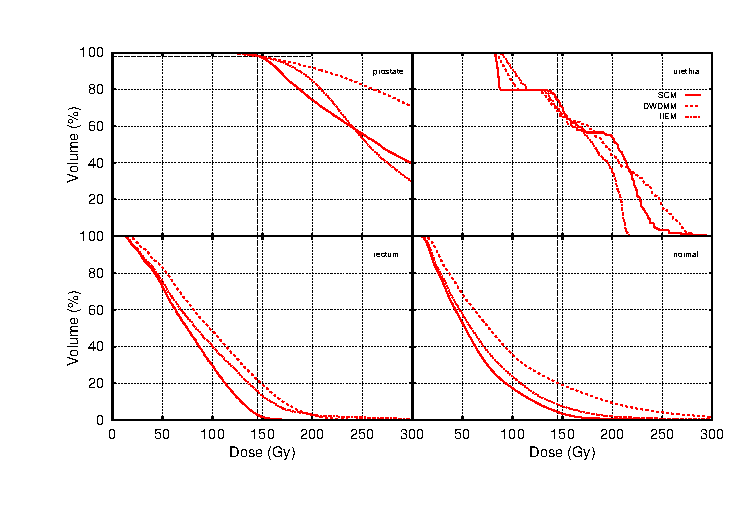
\includegraphics[width=4.3in]{figures/wiese-all4x4.pdf}
    \end{center}
  \end{figure}

\end{frame}

%%---------------------------------------------------------------------------%%
\begin{frame}{Patient O DVH Curves}
  
  \begin{figure}[h!]
    \begin{center}
      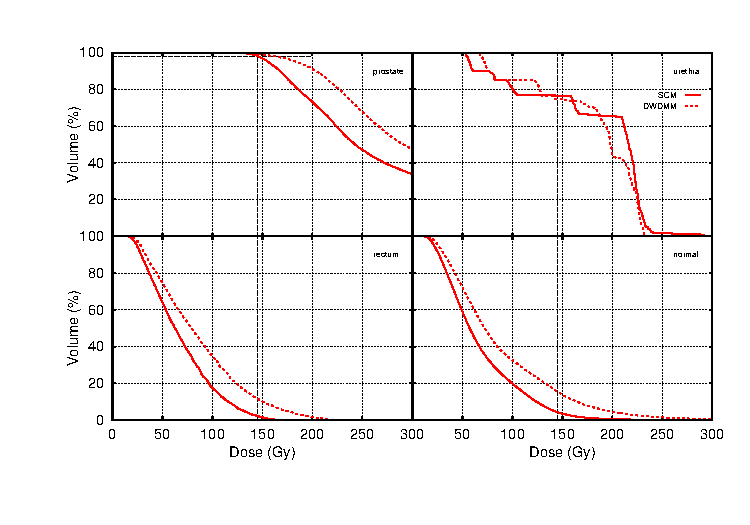
\includegraphics[width=4.3in]{figures/wollenburg_7_31_98-all4x4.pdf}
    \end{center}
  \end{figure}

\end{frame}

%%---------------------------------------------------------------------------%%
\begin{frame}{Patient P DVH Curves}
  
  \begin{figure}[h!]
    \begin{center}
      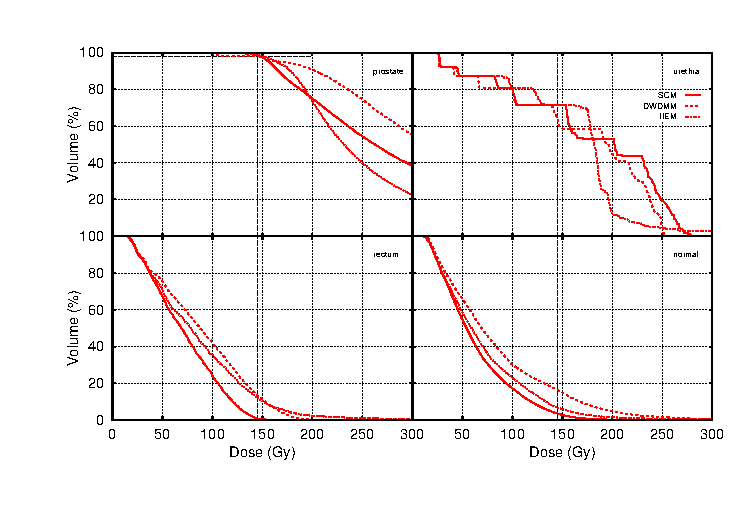
\includegraphics[width=4.3in]{figures/wray_7_10_98-all4x4.pdf}
    \end{center}
  \end{figure}

\end{frame}

%%---------------------------------------------------------------------------%%
\section{Conclusion}
%%---------------------------------------------------------------------------%%
\begin{frame}{Pros/Cons of Each Method}

  \begin{itemize}
    \item IIEM
      \begin{itemize}
        \item Pros:
          \begin{itemize}
            \item Very fast
            \item Does a good job of picking a small number of needles and
              seeds
            \item Does a good job of limiting prostate overdosing
          \end{itemize}
        \item Cons:
          \begin{itemize}
            \item Does not always converge (iterative)
          \end{itemize}
      \end{itemize}
      \medskip
    \item DWDMM
      \begin{itemize}
        \item Pros:
          \begin{itemize}
            \item Extremely fast 
            \item Guaranteed solution (non-iterative).
          \end{itemize}
        \item Cons:
          \begin{itemize}
            \item Tends to select a large amount of seeds
            \item Multiplication of the adjoint ratio by the dose does not have
              a physical motivation
          \end{itemize}
      \end{itemize}
  \end{itemize}

\end{frame}

%%---------------------------------------------------------------------------%%
\begin{frame}{Pros/Cons of Each Method}

  \begin{itemize}
    \item SCM
      \begin{itemize}
        \item Pros:
          \begin{itemize}
            \item Does a good job of picking a small number of seeds
            \item Does a good job of sparing sensitive tissues
            \item Motivated by a well established greedy heuristic from
              computer science
            \item Guaranteed solution (non-iterative).
          \end{itemize}
        \item Cons:
          \begin{itemize}
            \item Much slower than the other methods
            \item Tends to select a large number of needles
          \end{itemize}
      \end{itemize}
  \end{itemize}

\end{frame}

%%---------------------------------------------------------------------------%%
\begin{frame}{Future Work}

  \begin{itemize}
    \item Add support for directional seeds.
      \medskip
    \item Add support for other types of treatment planning.
      \medskip
    \item Suggestions?
  \end{itemize}

\end{frame}

\end{document}

